\documentclass[11pt,a4paper,oneside]{article}
%\documentclass[a4paper]{scrartcl}

\usepackage{geometry}
 \geometry{
 a4paper,
 total={210mm,297mm},
 left=20mm,
 right=20mm,
 top=20mm,
 bottom=20mm,
 }
 
\usepackage{enumitem}
\usepackage{color}
\def\red{\textcolor{red}}
\usepackage{titling}
\newcommand{\subtitle}[1]{%
  \posttitle{%
    \par\end{center}
    \begin{center}\large#1\end{center}
    \vskip0.5em}%
}

\usepackage{float}
\usepackage[english]{babel}
\usepackage[utf8x]{inputenc}
\usepackage{amsmath}
\usepackage{graphicx}
\usepackage[colorinlistoftodos]{todonotes}

\title{Topic Modelling using Latent Dirichlet Allocation}
\subtitle{CSE 250B Project 3}
\author{Suvir Jain, Gaurav Saxena}
\date{27 February,2014}

\begin{document}
\maketitle

\begin{abstract}
Abstract about LDA, our data, brief results.
\end{abstract}

\section{Introduction}

The objective of the project is to learn a Latent Dirichlet Allocation (LDA) model to predict dominant topics associated with a collection documents. This process is called topic modelling.

We discuss the LDA framework for topic modelling in section \ref{sec:Framework}. We, then, describe our implementation of algorithm based on the framework in section \ref{sec:Algorithms}. Furthermore, we discuss our experiments and code optimizations in \ref{sec:Experiments} and finally present results in \ref{sec:Results} and lessons learnt in section \ref{Lessons}

We use two data sets classic 400[\red{reference}] and hookah data set [\red{reference}] for topic modelling. We use Latent Dirichlet Allocation to discover latent topics in these data set. The latent variables are discovered using Collapsed Gibbs (CGS) Sampling.

We found 3 main themes in the classic400 data set. They are about biology, aeronautical science and a collection of research related words. 

In the hookah data set, we discovered that hookah related tweets have a social aspect to them. People commonly used words like 'party','bar','lol','tonight'  in their tweets.

\section{Framework}
\label{sec:Framework}

\subsection{Dataset}

\paragraph{Classic400}

This dataset is a part of classic3\cite{banerjee2005clustering} dataset. Classic3 dataset is a collection of 3893 documents, which in turn contains 1400 CRANFIELD documents from aeronautical systems papers, 1033 MEDLINE documents from medical journals and 1460 CISI documents from information retrieval papers. Classic400 is a collection of 400 documents randomly chosen from classic3 dataset by \cite{banerjee2005clustering}. We use the same dataset for our analysis.

This data set contains a total of 6505 words and hence each document is converted to a vector of 6505 integers, each showing the frequency a word in a document. The dataset also contains true labels of the dataset which we use for sanity check of our model. The dataset also contains the vocabulary used in the classic400. We use the vocabulary to find the top words for each topic.

\paragraph{Hookah data set}
This data set consists of a set of tweets about Hookah usage. These tweets are drawn from a larger collection of tweets. The main set of tweets was collected between November 2011 and August 2013 using the Twitter Application Programming Interface (API). These tweets represented 1\% of all tweets on Twitter during this time interval. On average, this data set consisted of 1.3 million tweets per day. Hookah-related tweets were extracted from this set using the keywords: hookah,hooka,waterpipe,shisha,sheesha and water pipe.The hookah data set consisted of 95,738 tweets. 

To allow for experiments to be done in a short amount of time, we could not use all 95,738 tweets. Hence, we extracted 3000 random tweets from this data set and used that for this project. This data set has a vocabulary size of 8021 words.

\paragraph{What did we expect to find?}
\subparagraph{Classic400 data set}
Our aim in processing this data set was to discover the dominant topics. Before running LDA, we did not have any idea about the themes and topics that characterize this data set. 

\subparagraph{Hookah data set}
This data set consists of tweets about hookah usage. We were interested in finding out the context in which people use hookah. Is it something people associate with negative emotions? Is it something that people use socially? Do people perceive hookah positively? Results are presented in section 5.2.2.

\subsection{Model}
\paragraph{Representation}
LDA uses a vector of length equal to the vocabulary to represent each document. Each element is represent the frequency of words found in that document. As discussed in class notes, this model is called bag of words. This representation doesn't preserve the word order and consequently loses information. However, as discussed in class notes, this representation may be sufficient to deduce topics from the documents. Therefore, for a document $d$ and a vector $\bar{x}$ then $x_j$ is the number of word $j$ in $d$ and the length of a document n is

\begin{equation}
	n = \sum^{m}_{j=1}x_j
\end{equation}

\paragraph{Multinomial Distribution over documents}
Now, given a set of documents and their representation as vectors, we need a model to represent them. A model is a probability distribution over the set of documents. We calculate the parameters of this model such that the training documents have a higher probability. We can, then, use this model to find the probability of a test document.

LDA uses multinomial distribution. Mathematical expression for a multinomial distribution is given below

\begin{equation}\label{multinomial}
p(x;\theta) = (\frac{n!}{\prod^m_{j=1}x_j!})(\prod^m_{j=1}\theta^{x_j}_j)
\end{equation}

where x is is a vector of non-negative integers and parameter $\theta$ are parameters of the model. In this expression, $\theta$ can be argued as a probability of a word $j$ while $x_j$ represents its count.

As discussed in the class notes, the first term in the equation \ref{multinomial}, the first term is the number of sentences which results in the same $x$ vector. The second term is the probability of an equivalence class of $\bar{x}$.

Also, given a set of training documents, the maximum likelihood estimate of the $j_{th}$ parameter is

\begin{equation}
\theta_j = \frac{1}{T} \sum_x x_j
\end{equation}

where the sum is over all documents x to the training set and $T = \sum_x{\sum_j{x_j}} $. However, this expression may lead to $0$ probabilities. Therefore, we add a constant to the expression called a pseudocount. It is a notional number of occurences of each word in each document. The formula, thus, becomes,

\begin{equation}
\theta_j = \frac{1}{T'} (c + \sum_x x_j)
\end{equation}

where $T' = mc + T$ and $0 < c \leq 1 $

\paragraph{Generative Process}
As discussed in the notes, the generative process assumes that the data points are generated by a probabilistic process. It helps to find the parameters of this process by based on the concept of maximum likelihood. The algorithm for the generative process is given in the notes\cite{classNotes} and not reproduced here for brevity. The generative process gives the following global probability distribution which represents a mixture distribution

\begin{equation}
f(x) = \sum^K_{k=1}f(x;\phi_k)
\end{equation}

where $x$ is a document, $\phi_k$ is a parameter value of the $k_{th}$ multinomial and $\alpha_k$ is the proportion of component number k.

In LDA we use Dirichlet Distribution which acts as a prior for multinomial distribution discussed above. It takes the following form \cite{classNotes}

\begin{equation}
p(\gamma|\alpha) = \frac{1}{D(\alpha)}\prod^m_{s=1}\gamma^{\alpha_s - 1}_s
\end{equation}

where ${D(\alpha)} = \int_\gamma \prod^m_{s=1}\gamma^{\alpha_s - 1}_s$

\subsubsection{Training Methods for LDA}

We use the words of the documents as our training data. We assume that the number of topics K, $\alpha$ and $\beta$ are fixed. Our aim is to learn $\theta$ values for documents and $\phi$ values topics. We use collapsed Gibbs Sampling for this process.

\paragraph*{Collapsed Gibbs Sampling}

As discussed in the class notes \cite{classNotes}, we use a variant of Gibbs Sampling called collapsed Gibbs Sampling (CGS) for learning the topics from the documents. In this process we do not try to learn $\theta$ and $\phi$ directly, but try to learn the hidden topic label $z$ for each word in each document.

We represent each word by its position in the document vector and its count as the value of the element at the position. However, CGS is based on the occurrence of the words. Therefore, the length of the z is taken as the sum of all the elements of the vector (or the length of the document).

Gibbs Sampling assumes that we know the $z$ value for an occurrence of word $i$. It, then, draws a random value of topic for every word except $i$ according to a distribution. We use the following distribution for Gibb's Sampling

\begin{equation}
p(z_i|\bar{z}', \bar{w}) = \frac{p(\bar{w} | \bar{z}) p(\bar{z})}{p(w_i|\bar{z}')p(\bar{w}'|\bar{z}')p(\bar{z}')}
\end{equation}

where $\bar{w}$ is the sequence of words of the vocabulary, $\bar{z}$ is the corresponding sequence of z values, $\bar{w}'$ represents $\bar{w}$ without the word $w_i$ and similarly, $\bar{z}'$ represents $\bar{z}$ without the word $w_i$. This expression can be reduced in terms of the counts of topics as given below

\begin{equation}
\label{prob}
p(z_i = j | \bar{z}', \bar{w}) = \frac{q_{j w_{i}'} + \beta_{w_i}}{\sum_t{q_{jt}' + \beta_t}}\frac{n_{mj'} + \alpha_j}{\sum_k{n_{mk}' + \alpha_k}}
\end{equation}

where $q_{j w_i}$ is the count of word $w_i$ occurs with topic $j$, $q_{j w_i}'$ is the count of word $w_i$ occurs with topic $j$ except for the word $w_i$, $n_{mk}$ is the count of the number of times topic $z_i = k$ in the document $m$ and $n_{mk}'$ is the count of the number of times topic $z_i = k$ in the document $m$ except for the word $w_i$ 

\subsubsection{Topic Metrics from LDA}
The aim of the CGS is to come up with words which together give shape to a topic. This is done by first finding dominant topics using $\theta$ values and then finding the words which provides context for this topic using $\phi$ values. 

$\theta$ values are a measure of probabilities that a document aligns with a topic. Therefore, dominant topics can be found by finding the topics which have the most documents associated with it. This is done by finding the maximum $\theta$ value for each document. Dominant topics can be found by keeping a count of the documents associating with a topic. This is discussed in detail in section \ref{sec:Algorithms}.

Similarly, words with highest $\phi$ values for a topic are expected to be associated with a topic. We pick top 10 words with the highest $\phi$ values for each topic. The details can be found in \ref{sec:Algorithms}.

\section{Design and Analysis of Algorithms}
\label{sec:Algorithms}

Mention complexities of algorithms.

\subsection{LDA Initialization}
We run topic modelling on two aforementioned datasets to find the dominant topics for each. As discussed in the class notes \cite{classNotes}, we initialize $z$ as a $M \times N_m$ array. A $z_i$ represents a position of a word in a sentence. Therefore, each word may occur multiple times in $z$. We assign topics randomly to all $z$ values.  Subsequently, using the corpus we initialize $q$ as a $K \times V$ based on z and the corpus. Similarly, we also initialize $n$ counts as a $K \times M$ using z and the corpus. The complexity of this process is $O(MN_m)$.

We also initialized the number of topics $K$, pseudocounts $\alpha$ and $\beta$ before the modeling.

\paragraph{Chosing $K$, $\alpha$, $\beta$}
Choice of $K$, $\alpha$, $\beta$ is critical a directly affects the quality of topics and the words association. High $\beta$ values tend to decrease the number of topics as it reduces the impact of sparsity \cite{griffiths2004finding}. This is a important for our case, in particular, as we are dealing with small number of themes in both classic400 datasets and hookah. Therefore, as advised by \cite{griffiths2004finding} we use $\beta = 0.1$. 

Similarly, $\alpha$ is used to for smoothing the $\theta$ distribution. It adds contribution from each topic to each document. Therefore, high values for $\alpha$ can reduce the separation between different topics and can lead to smudging of boundaries between them. We chose $\alpha = 50/K$ as suggested in the class and in \cite{griffiths2004finding}.

Although, we assume both $\alpha$ and $\beta$ to be constant but they can be found using EM algorithm. However, this increases the run time of the algorithm and therefore we have not implemented it.

Knowing $\alpha$ and $\beta$, the values of $K$ can be found by maximizing the likelihood of data, as suggested by \cite{griffiths2004finding}. In their experiments they found that $K = 300$ to be a value at which likelihood peaks. However, we did not follow this procedure as we are not expecting a large number of topics and calculating likelihood computation is not computationally trivial. We experimented with several value of K and qualitatively found that noise words reduced with increasing K in dominant topics.

\subsection{Collapsed Gibb's Sampling}
We ran Collapsed Gibbs Sampling to convergence to find the dominant topics of the corpus. To achieve this we used equation \ref{prob} for an estimate of probability \cite{classNotes}. It is reproduced here for clarity.

\begin{equation}
p(z_i = j | \bar{z}', \bar{w}) = \frac{q_{j w_{i}'} + \beta_{w_i}}{\sum_t{q_{jt}' + \beta_t}}\frac{n_{mj'} + \alpha_j}{\sum_k{n_{mk}' + \alpha_k}}
\end{equation}

For each document, and each position (a word could take) in the document, we calculated probability of each topic being assigned to the position. We assumed that the current topic assigned to the position was fixed and calculated the probability estimate using equation \ref{prob} of all the topics for this position. We, then, randomly selected a topic using the distribution of the these probability estimates.

We did this for each position and a number of iterations until the $z$ values stopped changing by a wide margin at which point we assumed that convergence is reached

\subsection{Obtaining Topics}
Once we the final values of z, we calculated $\theta$ and $\phi$ values to get the topics and words associated with the them. We used the following equations \cite{classNotes} to do it

\begin{equation}
\hat{\theta_k} = \frac{\sum^M_{i=1}{I(z_i=k)}}{n}
\end{equation}

\begin{equation}
\hat{\phi_kj} = \frac{\sum^M_{d=1}{\sum^{n_d}_{i=1}{I(w_i=j \land z_i = k)}}}{\sum^M_{d=1}{\sum^{n_d}_{i=1}{I(z_i = k)}}}
\end{equation}

where $z_i$ is the topic-word association vector, $w_i$ is  a word, $k$ is a topic, $M$ is the number of documents, $n_d$ is the length of a document $d$.

Topics with the highest $\theta$ values were taken as dominant topics. Although we ran for various $K$ values but we considered only top 3 dominant topics as we conjectured that both classic400 and hookah datasets have a small number of dominant themes and as we present in the results, probabilities of other topics was too low to be considered.

\subsection{Topic Metrics}
Furthermore, we collected more information for reporting like top words, document and word coverage for each topic. Top 10 words were calculated by taking the $argmax$ of the top 10 $\phi$ value for a topic. \textit{Document coverage} is a ratio of the number of documents with a specific topic to the total number of topics. Similarly, \textit{word coverage} is a ratio of the number of words associated with a topic to the total number of topics.

\section{Design of Experiments}
\label{sec:Experiments}

\subsection{Dataset Preprocessing}
Pre-processing was required only for the second data-set. The classic400 dataset was used as provided in the \textsc{Matlab} file format.

The following steps were taken to pre-process the hookah data set : 

\begin{enumerate}
  \item The text is tokenized using the Punkt Tokenizer \cite{punkt} which is part of the Python NLTK library \cite{nltk}. This process splits the tweets into individual words.
  \item Then, the tokens are stemmed using the Porter Stemmer \cite{porter}, also part of the Python NLTK library. This helps map similar words to the same stem. Word variations like plurals and tense-based conjugates are replaced by the root word.
  \item All stopwords were deleted. Stopwords are common words like 'I' ,'me',can' etc. We used a list of 127 stopwords that is provided with NLTK\cite{nltk}.
  \item All words are mapped to unique integer values and represented in the same format as classic400 i.e. a matrix of dimensions K(number of documents) x V(size of vocabulary).
\end{enumerate}

Mention the stopwords used for processing second dataset.
Cite the link : http://cseweb.ucsd.edu/users/elkan/151/classic400.mat

\subsection{Experiments with LDA}
We ran the LDA implementation on both data sets for different number of topics. Specifically, we experimented with K = 3,10,50,100. 

For each experiment, the $\theta$ vector and $\phi$ vector were recorded. From these, we inferred the top 3 topics for the entire data set. The top 3 topics are the 3 topics with which the highest number of words and documents were labeled.

We also tracked the number of topic-word associations that remained the same between consecutive iterations of LDA. This measure served as a indicator of convergence of the distribution. Related plot are presented in the results section.

\subsection{Implementation}
We implement LDA in \textsc{MATLAB}.

The pre-processing code was written in Python. Specifically, the NLTK python library was used for tokenizing, stemming and removing stop words. Details of these procedures are covered in section 4.1.

Some more implementation details that we discovered while developing the code are :

\begin{enumerate}
  \item \red{Z is specific to a document. Therefore it will have a different length for different document.}
  \item \red{Also each word can have a different topic, therefore there will be a different entry for each word in Z. However, this is not true about q and n as they are counts. They will have K * V and K * M sizes.}
\end{enumerate}

\subsection{Code Optimization}
We optimized the following equation in 4 ways :

\begin{equation}
p(z_i = j | \bar{z}', \bar{w}) = \frac{q_{j w_{i}'} + \beta_{w_i}}{\sum_t{q_{jt}' + \beta_t}}\frac{n_{mj}' + \alpha_j}{\sum_k{n_{mk}' + \alpha_k}}
\end{equation}

\begin{enumerate}
\item $q_{j w_{i}'}+\beta_{w_i}$ In this part of the calculation, $\beta_{w_i}$ is constant for any fixed value of j. Therefore, for each j, $\beta_{w_i}$ were added it to all $q_{j w_{i}'}$ outside the loop. 
\item $n_{mj}' + \alpha_j$ For each value of j, $\alpha_j$ is a constant. Therefore, for each j, $\alpha_j$ was added to all $n_{mj}'$ outside the loop.
\item $\sum_t{q_{jt}' + \beta_t}$ For any value of t, $\beta_t$ is a constant value. Therefore, for all t, $\beta_t$ was added to $\sum_t{q_{jt}}'$.
\item $\sum_k{n_{mk}' + \alpha_k}$ For any value of k, $\alpha_k$ is a constant. Therefore, for all k, $\alpha_k$ is added to all $\sum_k{n_{mk}}'$.
\end{enumerate}

\bigskip
One more code optimization saved us a lot of time during experiments. This was in the calculation of the $\phi$ vector. Calculating the $\phi$ vector for all topics is an O(K*V*M) operation. V and M cannot really be optimized. However, we did optimize the K value. We calculated $\phi$ vector for only the top 3 topics. These top 3 topics were the topics with which most documents were associated as per the $\theta$ vector.


\subsection{Sanity Checks}
We used the following checks during the development of the code to ensure that our implementation was correct.
\begin{enumerate}
\item For the classic400 dataset, we had access to the true labels which were grounded in real-world truth. We compared the topic distribution of our learned model to these true labels. 
\item After initializing q and n, the sum of these two vectors should be the same and it should equal the total number of words in the corpus.
\end{enumerate}

\section{Results of Experiments}
\label{sec:Results}

\subsection{Convergence of LDA}
In order to measure the convergence of LDA, we tracked the word-topic associations recorded by vector z. After each iteration, we measured the number of z values which had stayed the same. 

This measure($\Delta z$) stabilized after some iterations. This experiment was repeated for number of topics K = 3,10,50,100. 

The \ref{fig:classic400_convergence} shows this convergence for classic400 data set. The \ref{fig:hookah_convergence} shows this convergence for hookah data set.

\begin{figure}[H]
\centering
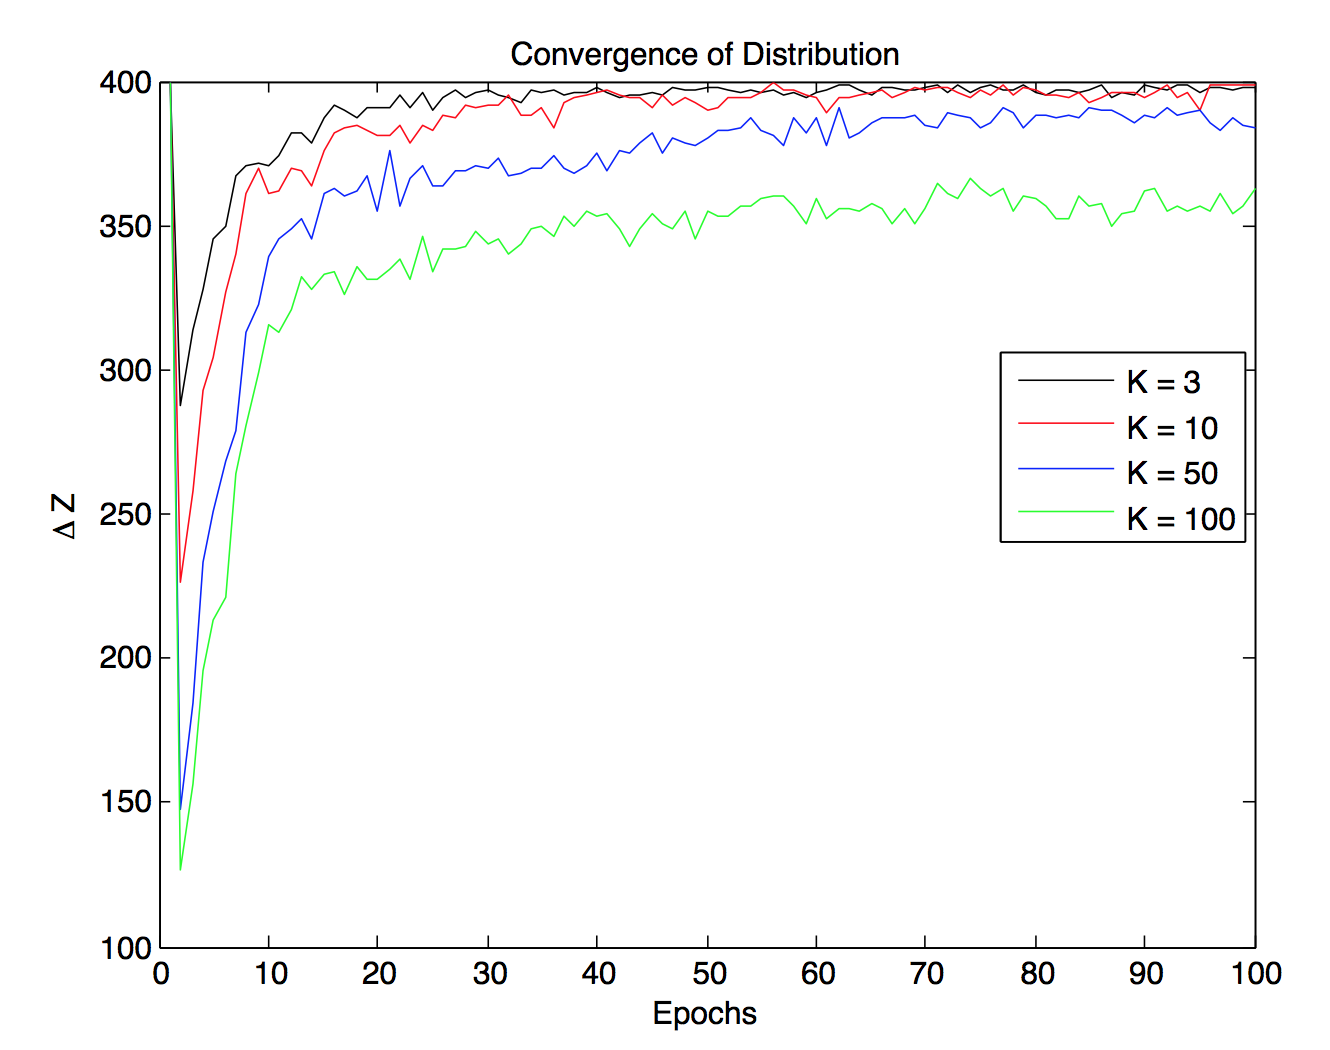
\includegraphics[width=\columnwidth]{classic400_convergence}
\caption{Tracking the convergence of LDA over 100 iterations for classic400 data set.}
\label{fig:classic400_convergence}
\end{figure}

\begin{figure}[H]
\centering
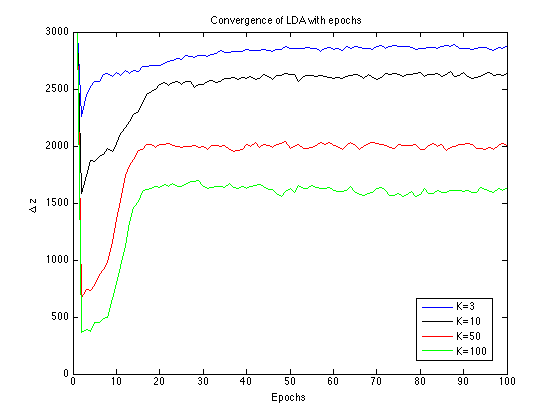
\includegraphics[width=\columnwidth]{hookah_convergence}
\caption{Tracking the convergence of LDA over 100 iterations for Hookah data set.}
\label{fig:hookah_convergence}
\end{figure}

\subsection{Topic Models discovered}
\subsubsection{Classic400 data set}
The tables \ref{table:k=3_classic400},\ref{table:k=10_classic400},\ref{table:k=50_classic400},\ref{table:k=100_classic400} shows the topic models discovered by LDA for the classic 400 data set with K = 3, 10, 50 and 100, respectively. 

We found 3 dominant topics in the classic400 data set. 
\begin{enumerate}
\item The first topic has words related to aviation and aeronautical engineering. For example - mach, supersonic, wings, and velocity.
\item The second topic has words like scientific, research, language, and methods. These keywords seem to be related to scientific research and pulications.
\item The third topic has medical terms like ventricular, left, aortic, and septal. All these terms are commonly used in medical science.
\end{enumerate}

\begin{table}
\begin{tabular}{|c|c|c|c|}
\hline 
Topic & Words & Document Coverage (\%) & Word Coverage(\%) \\ 
\hline 
1 & boundary,layer,wing,mach,supersonic, & 50.25 & 38.07 \\ 
  & ratio,wings,velocity,effects,shock & & \\
\hline 
2 & patients,ventricular,left,retrieval,cases, & 15.75 & 38.53 \\ 
  & system,language,aortic,septal,research & & \\
\hline 
3 & fatty,acids,glucose,journals,acid & 34 & 23.40 \\ 
 & ffa,free,blood,nickel,infants & & \\
\hline
\end{tabular}
\caption{Topics Discovered in classic400 data set for K=3}
\label{table:k=3_classic400}
\end{table}

\begin{table}
\begin{tabular}{|c|c|c|c|}
\hline 
Topics & Words & Document Coverage(\%) & Word Coverage(\%) \\ 
\hline 
 1 & boundary,layer,wing,mach,supersonic,ratio & 0.4975 & 56.15 \\ 
& wings,velocity,effects,shock & & \\
\hline 
 2 & system,scientific,retrieval,research,language & 0.2475 & 23.38 \\
& science,journals,systems,methods,subject & & \\ 
\hline 
 3 & patients,ventricular,left,aortic,septal,cases, & 0.1025 & 20.47 \\ 
& defect,regurgitation,ventricle,pulmonary & & \\
\hline 
\end{tabular}
\caption{Topics Discovered in classic400 data set for K=10}
\label{table:k=10_classic400}
\end{table}

\begin{table}
\begin{tabular}{|c|c|c|c|}
\hline 
Topics & Words & Document Coverage(\%) & Word Coverage(\%) \\ 
\hline 
 1 & boundary,layer,wing,mach,supersonic, & 50.00 & 58.97 \\ 
& ratio,wings,effects,velocity,shock & & \\
\hline 
 2 & system,scientific,retrieval,research,language, & 23.75 & 19.47 \\ 
& science,systems,journals,subject,requests & & \\
\hline 
3 & patients,ventricular,left,cases,aortic,septal, & 12.75 & 21.56 \\ 
& defect,regurgitation,ventricle,pulmonary & & \\
\hline 
\end{tabular}
\caption{Topics Discovered in classic400 data set for K=50}
\label{table:k=50_classic400}
\end{table}

\begin{table}
\begin{tabular}{|c|c|c|c|}
\hline 
Topics & Words & Document Coverage(\%) & Word Coverage(\%) \\ 
\hline 
1 & boundary,layer,wing,mach,supersonic,ratio & 56.75 & 68.51 \\ 
& wings,effects,velocity,shock & & \\
\hline 
2 & patients,ventricular,left,cases,aortic,septal, & 14.00 & 20.27 \\ 
& visual,defect,regurgitation,ventricle & & \\
\hline 
3 & retrieval,language,system,subject,systems, & 10.50 & 11.22 \\ 
& library,requests,descriptor,basic,search & & \\
\hline 
\end{tabular}
\caption{Topics Discovered in classic400 data set for K=100}
\label{table:k=100_classic400}
\end{table}

\subsubsection{Hookah data set}
The tables \ref{table:k=3_hookah},\ref{table:k=10_hookah},\ref{table:k=50_hookah},\ref{table:k=100_hookah} shows the topic models discovered by LDA for the Hookah data set with K = 3, 10, 50 and 100, respectively. 

We found that the hookah tweets were dominated by a words like smoke, bar, 'lol', 'like','tonight'.

This was in line with our hypotheses that Hookah is normally associated with positive emotions and is used in a social context. 

Some interesting points to note about the discovered keywords in this data set :
\begin{enumerate}
\item 'http' is a word in the dominant topic. This is used in tweets when people 're-tweet' or RT. RTs typically have a short URL.
\item Words like 'combinado', 'fumando', 'una' are seen in the keyword list. These are spanish words. The data set has a mixture of english and non-english tweets.

These results reinforce the findings of prior work by Myslin et al \cite{JMIR}. Their work had indicated that some tobacco products are perceived positively. These products provide opportunities for tobacco control education.

\end{enumerate}

\begin{table}
\begin{tabular}{|c|c|c|c|}
\hline 
Topic & Words & Document Coverage(\%) & Word Coverage(\%) \\ 
\hline 
1 & hookah,http,shisha,smoke,bar, & 79.23 & 56.89 \\ 
& hooka,lol,like,night,tonight & & \\
\hline 
2 & shisha,party,que,hookah,con, & 11.77 & 24.21 \\ 
& http,una,die,fumando,fumar & & \\
\hline 
3 & shisha,haha,aku,rokok,tak, & 9.00 & 18.90 \\ 
& nak,hisap,sheesha,hahaha,yang & & \\
\hline 
\end{tabular}
\caption{Topics Discovered in Hookah data set for K=3}
\label{table:k=3_hookah}
\end{table}

\begin{table}
\begin{tabular}{|c|c|c|c|}
\hline 
Topics & Words & Document Coverage(\%) & Word Coverage(\%) \\ 
\hline 
1 & hookah,http,shisha,smoke,bar, & 76.57 & 71.41 \\ 
& hooka,lol,like,night,tonight & & \\
\hline 
2 & shisha,haha,aku,tak,rokok, & 10.67 & 0.1905 \\ 
& hahaha,die,nak,hisap,dia & & \\
\hline 
3 & party,que,con,una,vamoc, & 3.90 & 0.954 \\ 
& party,por,fumando,esta,sheesha & & \\
\hline 
\end{tabular}
\caption{Topics Discovered in Hookah data set for K=10}
\label{table:k=10_hookah}
\end{table}

\begin{table}
\begin{tabular}{|c|c|c|c|}
\hline 
Topics & Words & Document Coverage(\%) & Word Coverage(\%) \\ 
\hline 
1 & hookah,shisha,http,smoke,bar, & 70.60 & 94.22 \\ 
& hooka,lol,like,night,tonight & & \\
\hline 
2 & party,hooka,thank,para,que, & 1.07 & 3.07 \\ 
& pra,combinado,right,power,move & & \\
\hline 
3 & club,hai,grandma,haram,hahaha, & 0.87 & 2.72 \\ 
& go,homi,super,till,good & & \\
\hline 
\end{tabular}
\caption{Topics Discovered in Hookah data set for K=50}
\label{table:k=50_hookah}
\end{table}

\begin{table}
\begin{tabular}{|c|c|c|c|}
\hline 
Topic & Words & Document Coverage(\%) & Word Coverage(\%) \\ 
\hline 
1 & hookah,shisha,http,smoke,bar, & 61.10 & 97.24 \\ 
& hooka,lol,like,night,loung & & \\
\hline 
2 & shisha,hookah,boy,ligero,rene,fri, & 0.73 & 1.45 \\ 
& offer,time,party,catchaflight & & \\
\hline 
3 & hookah,heart,http,talk,hooka,wine, & 0.7 & 1.31 \\ 
& satelit,dgib,shower,mypoorlung & & \\
\hline 
\end{tabular}
\caption{Topics Discovered in Hookah data set for K=100}
\label{table:k=100_hookah}
\end{table}


\subsection{Plot of $\theta$ vector}
We evaluated the theta vector as described in section 2.2.

This was done for both the data sets and visualized in plots. These plots help visualize the documents clustered by their most likely topics. 

It is interesting to see that most documents align themselves in 3 clusters. The topics which dominate have dense clusters and other topics have a sparse cluster.

Fig. \ref{fig:triangle_classic400} and Fig. \ref{fig:triangle_hookah} are plots of the $\theta$ vector for the classic400 and hookah data set, respectively. They helps in visualizing the hyperplane between topics. 

Fig. \ref{fig:scatter_classic400} and Fig. \ref{fig:scatter_hookah} are plots of the $\theta$ vector but in scatter plot form. These plots helps to visualize the documents clustered by topics.

\begin{figure}[H]
\centering
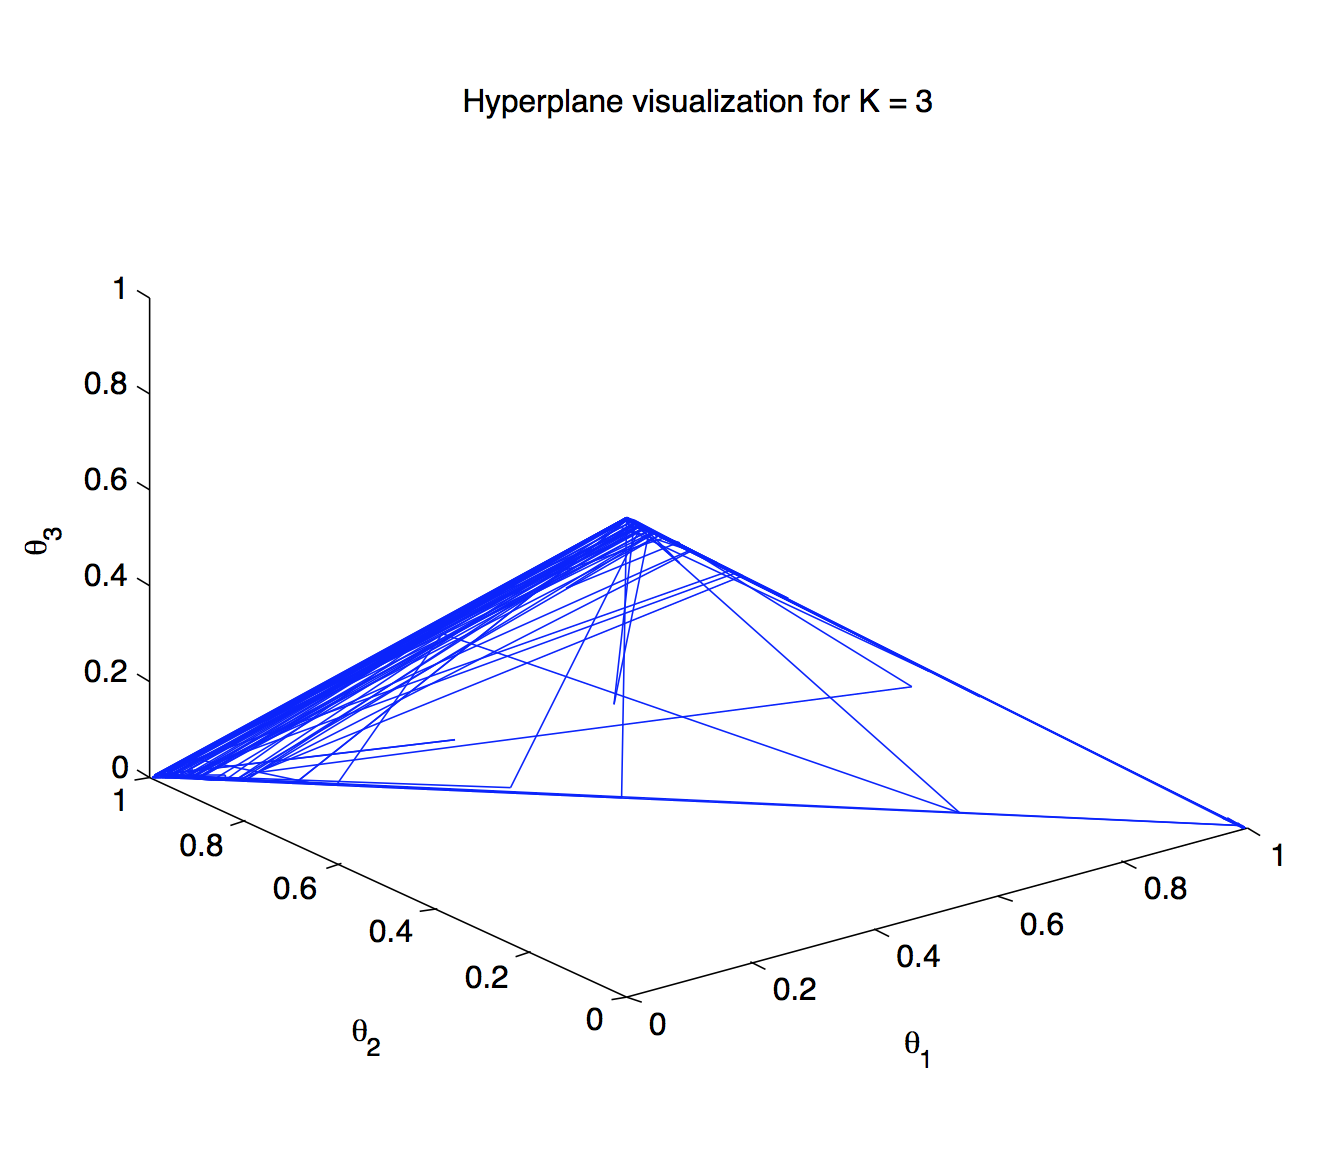
\includegraphics[width=\columnwidth]{triangle_classic400}
\caption{classic400 : Plot of $\theta$ vector helps in visualizing the documents clustered by topics}
\label{fig:triangle_classic400}
\end{figure}

\begin{figure}[H]
\centering
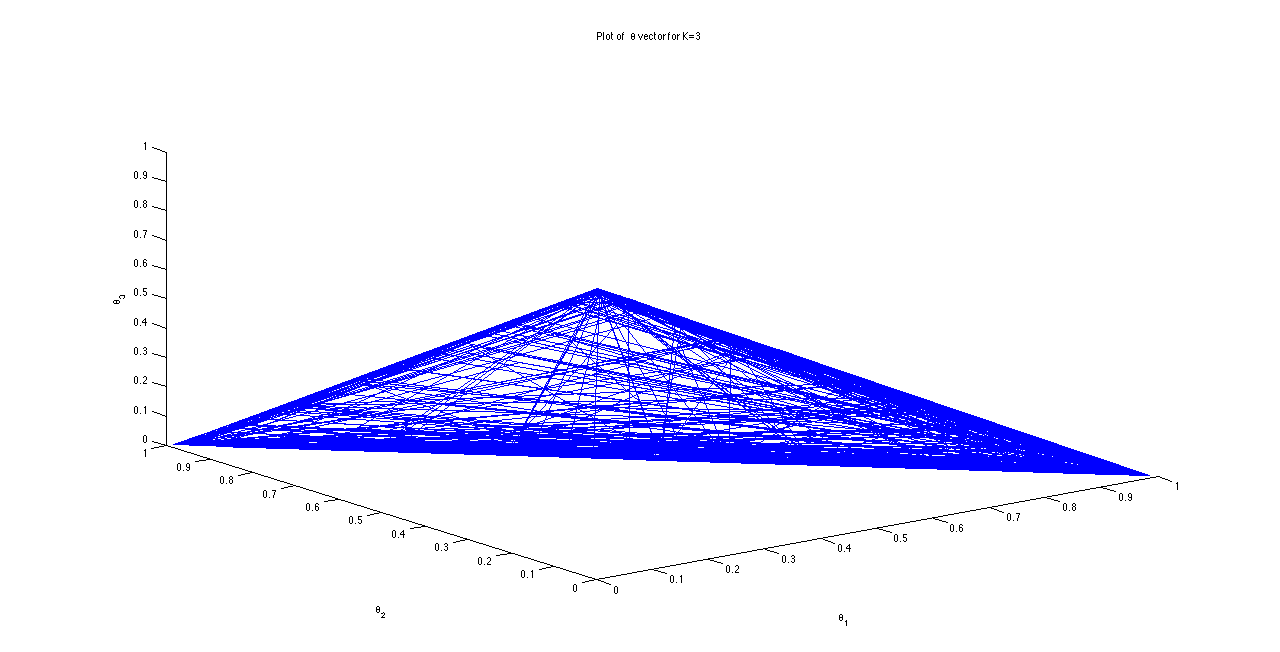
\includegraphics[width=\columnwidth]{triangle_hookah}
\caption{Hookah data set : Plot of $\theta$ vector helps in visualizing the documents clustered by topics}
\label{fig:triangle_hookah}
\end{figure}

\begin{figure}[H]
\centering
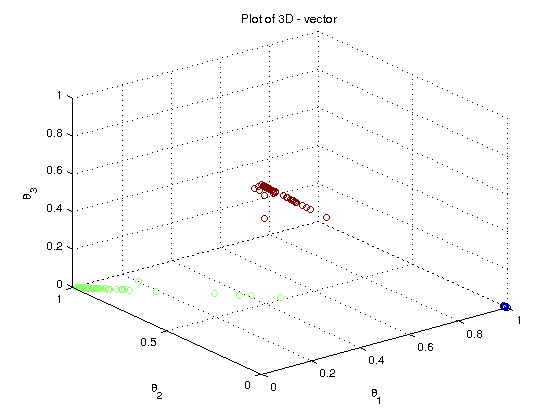
\includegraphics[width=\columnwidth]{scatter_classic400}
\caption{Classic400 : Visualizing documents clustered by topics}
\label{fig:scatter_classic400}
\end{figure}

\begin{figure}[H]
\centering
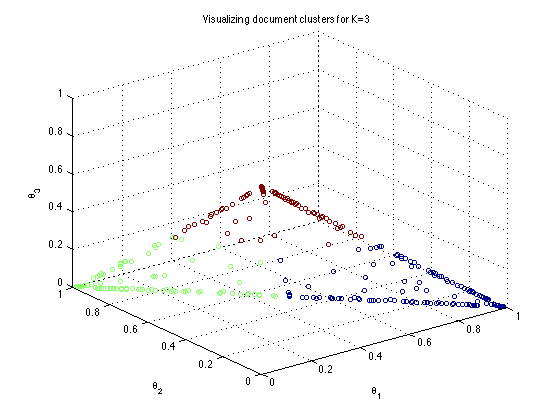
\includegraphics[width=\columnwidth]{scatter_hookah}
\caption{Hookah Data Set : Visualizing documents clustered by topics.}
\label{fig:scatter_hookah}
\end{figure}

\subsection{Comparison with true labels in classic400 data set}
For the classic400 data set, we have access to the set of true labels based on real-world knowledge. Fig. \ref{fig:truelabels} plots the number of documents labelled by each topic. This plot is superimposed over the number of documents labelled by the true labels. We see that discovered topics closely track the true labels.

\begin{figure}[H]
\centering
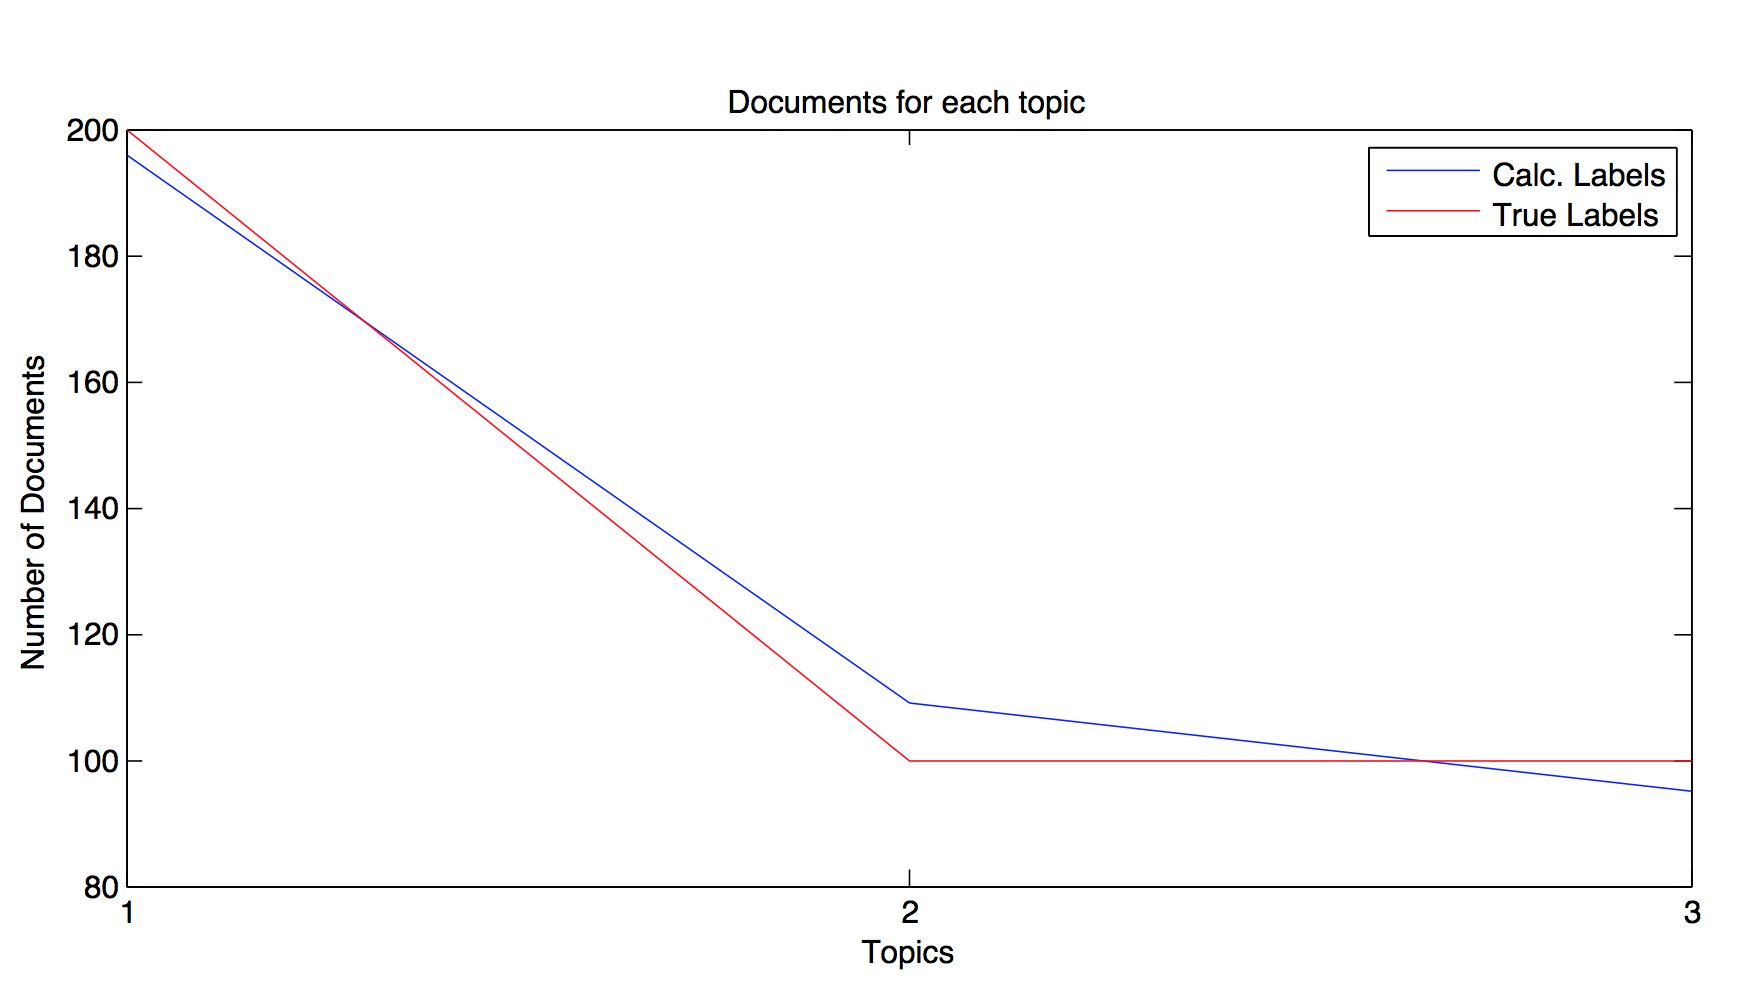
\includegraphics[width=\columnwidth]{truelabels}
\caption{Classic400 : Topics discovered by LDA vs True Labels}
\label{fig:truelabels}
\end{figure}

\section{Lessons Learned}
\label{Lessons}
\begin{itemize}
\item The main bottleneck in running the code was its slow speed of Collapsed Gibbs Sampling. We started with a running time of more then 2 hours for 100 iterations on Haskel i5, 4GB machine. After the optimizations done in \ref{Lessons} we could complete 100 iterations in about 30 minutes.
\item We found that calculation of LCL is computationally expensive. Therefore, as a measure of convergence we tracked change in the distribution during the iterations of CGS. We found that when the number of z values stop changing, there was a good separation in the topics.
\item Evaluating quality of a topic model is a subjective thing. \cite{chang}
\item We also found that having less number of topics than the actual gives incoherent word-topic matches. However, as the number of topics increase this incoherence decreases. Even when the number of topics is more than true topics, the dominant topics still emerge and we found that with increasing $K$ the word-topic associations still stay the same.
\end{itemize}

\subsection{Goodness of Fit}
We did a brief survey of literature about goodness of fit of LDA models. It appears that defining goodness of fit for LDA is a non-trivial and rather tricky task \cite{heinrich},\cite{nguyen}.

\subsubsection{Defining goodness of fit}
As per \cite{nguyen}, if the topics $\phi_{1}$ to $\phi_{k}$ are given, the goodness-of-fit can be modeled as $p(\bar{w}| \Phi,\alpha )$. If the topics $\phi_{1}$ to $\phi_{k}$ are not available, the author suggests the goodness-of-fit can be modeled as $p(\bar{w}| \alpha,\beta )$, where $\alpha$ and $\beta$ are the hyperparameters of the LDA.

As per the Elkan \cite{perplexity}, perplexity can be used as a measure of goodness of fit. Perplexity is the reciprocal geometric mean of the likelihood of a test corpus :

\begin{equation}
P( \tilde{W} | Q) = \prod_{i=1}^M{p(\tilde{\bar{w}}_{\tilde{m}} | \alpha)}
\end{equation}

%\product_{i=1}^M{T}
%_{\tilde{m}}
\red{delete}
In the report, try to answer the following questions. The questions are related to each other, and do not have definitive answers.
1. What is a sensible way to define the goodness-of-fit, for the same dataset, of LDA models with different hyperparameters K, ALPHA, and BETA? (Refer to tips in class notes)
2. Given the definition of goodness-of-fit, is it possible to compute it numerically, either exactly or approximately?
3. How can we determine whether an LDA model is overfitting its training data?
For the two datasets with which you do experiments, present and justify good values for K, ALPHA and BETA. You can choose these values informally (you do not need an automated algorithm) but your choices should be sensible and justified.


\bibliographystyle{abbrv}
\bibliography{Report}

\end{document}
